\documentclass{standalone}
\usepackage{tikz}
\usepackage{ctex,siunitx}
\setCJKmainfont{Noto Serif CJK SC}
\usepackage{tkz-euclide}
\usepackage{amsmath}
\usetikzlibrary{patterns, calc,3d}
\usetikzlibrary {decorations.pathmorphing,decorations.pathreplacing,decorations.shapes}
\tikzset{label style/.append style={font=\small}}
\begin{document}
\small
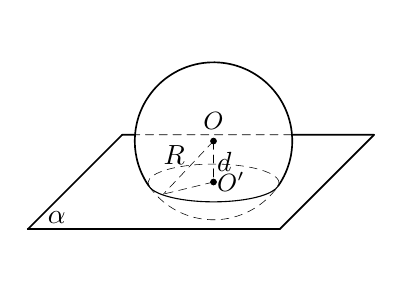
\begin{tikzpicture}[>=latex,scale=0.8,inner sep=1pt]
\useasboundingbox(0,-0.6)rectangle(5.5,3.2); 
  \tkzDefPoints{0/0/Q,4/0/M,5.5/1.5/N,1.5/1.5/P,2.95/0.75/O',2.95/1.4/O}
  \tkzDefShiftPoint[O](-145:1.25){R}
  \tkzDefShiftPoint[O](-35:1.25){R'}
  \tkzDefShiftPoint[O']({1.04*cos(-140)},{0.3*sin(-140)}){r}
  \tkzInterLC(N,P)(O,R)\tkzGetPoints{s}{s'}
  \tkzDrawSegments[semithick](P,Q Q,M M,N N,s s',P)
  \tkzDrawSegments[densely dashed](s,s' O,O' O,r O',r)
  \tkzDrawArc[densely dashed](O,R)(R')
  \tkzDrawArc[semithick](O,R')(R)
  \draw[densely dashed,very thin](R)arc(190:-10:1.04 and 0.3);
  \draw(R)arc(-170:-10:1.04 and 0.3);
  \tkzLabelLine[pos=0.5,right](O,O'){$d$}
  \tkzLabelLine[pos=0.5,above left](O,r){$R$}
  \tkzDrawPoints[fill=black](O,O')
  \tkzLabelPoints[above=3pt](O)
  \tkzLabelPoints[right](O')
  \tkzLabelAngle[pos=0.5](M,Q,P){$\alpha$}
\end{tikzpicture}
\end{document}